% !TEX root = ../thesis.tex
\chapter{Design Adaptations}\label{cha:designChanges}
For building the \gls{EDiC} the goal was to keep to the same basic infrastructure of the first version \gls{CPU}.
However, many bugs and problems that occurred in the building of it should be addressed and avoided.
Furthermore, the \gls{CPU} should be extended with some important features that were not implemented in the first version.
\section{General Improvements}\label{sec:improvements}
There are several design decisions, especially in the hardware built, which caused problems or could have caused problems in certain circumstances.
\paragraph{LED Driver}
First of all, all \glspl{LED} were directly connected to the logic wires.
This does work but the outputs of all logic \glspl{IC} have a limited current they can provide.
For example, the \emph{74LS245} is rated for maximum \qty{20}{\uA} for high-level output and \qty{-200}{\micro\ampere} for an low-level output \cite{74ls245}.
The way the \glspl{LED} were connected in the first \gls{CPU} they use only current when the logic \gls{IC} outputs a high-level voltage which is rated for \nicefrac{1}{10} the output current.
When connecting more \glspl{IC} and one \gls{LED} the maximum current can easily be exceeded.
Therefore, all \glspl{LED} of the \gls{EDiC} are powered with an additional inverting driver, the \emph{74ABT540} which is rated for \qty{50}{\uA} in both directions \cite{74abt540}.
\paragraph{Register \gls{IC}}
\begin{figure}[t]
  \centering
  \includegraphics[width=.6\textwidth]{ce.png}
  \caption{Clock Enable circuit of the \emph{74F825} \gls{IC} \cite{74f825}.}
  \label{fig:clockEnable}
\end{figure}
% A basic 1 bit register
The 74 series of logic \glspl{IC} feature many different registers.
The most basic register \gls{IC} has $n$ D-type flip-flops with respective data inputs and outputs plus one common clock input.
On each rising edge of the clock the flip-flops capture the input values and hold them until the next rising edge of the clock.
However, often it is required that a register does not capture on every rising edge of the clock.
This is done with an additional input, called clock enable.
In the first version of the \gls{CPU} the clock inputs of the registers that needed clock enable were connected to the output of an AND gate of the clock and a control bit.
This has the major drawback that glitches of the enable control signal can propagate to the clock input of the register when the clock is currently high.
There are two widely used alternatives to the simple AND gate:
The enable input can be used as the select input for an multiplexer to the data input of the flip flop, where it multiplexes between the actual input and the current output.
This allows the flip-flop to always capture data but when the enable input is inactive, it recaptures the current output.
The drawbacks are that each bit of the register needs a multiplexer at the input and secondly that the flip-flops draw power on every clock pulse, even though no data is captured.
The \emph{74F825} logic \gls{IC} solves this with the circuit shown in \cref{fig:clockEnable}.
When the $\overline{\text{EN}}$ input is low, the CP input is NAND gate on the right passed the negated CP through\footnote{The internal flip-flops of the \emph{74F825} are negative edge triggered}.
When the $\overline{\text{EN}}$ input is high, on the other hand, the output does not change.
This circuit prevents the $\overline{\text{EN}}$ to trigger a falling edge (which would trigger the flip-flops) on the CP output.
However, when the $\overline{\text{EN}}$ goes high while the CP input is high, then the output also goes high.
This is not directly a problem because the flip-flops only trigger on falling edges but is the reason for timing requirements on the $\overline{\text{EN}}$ input which are discussed in more detail in \cref{sec:timing}.
\begin{figure}[t]
  \centering
  \begin{subfigure}[b]{.45\textwidth}
    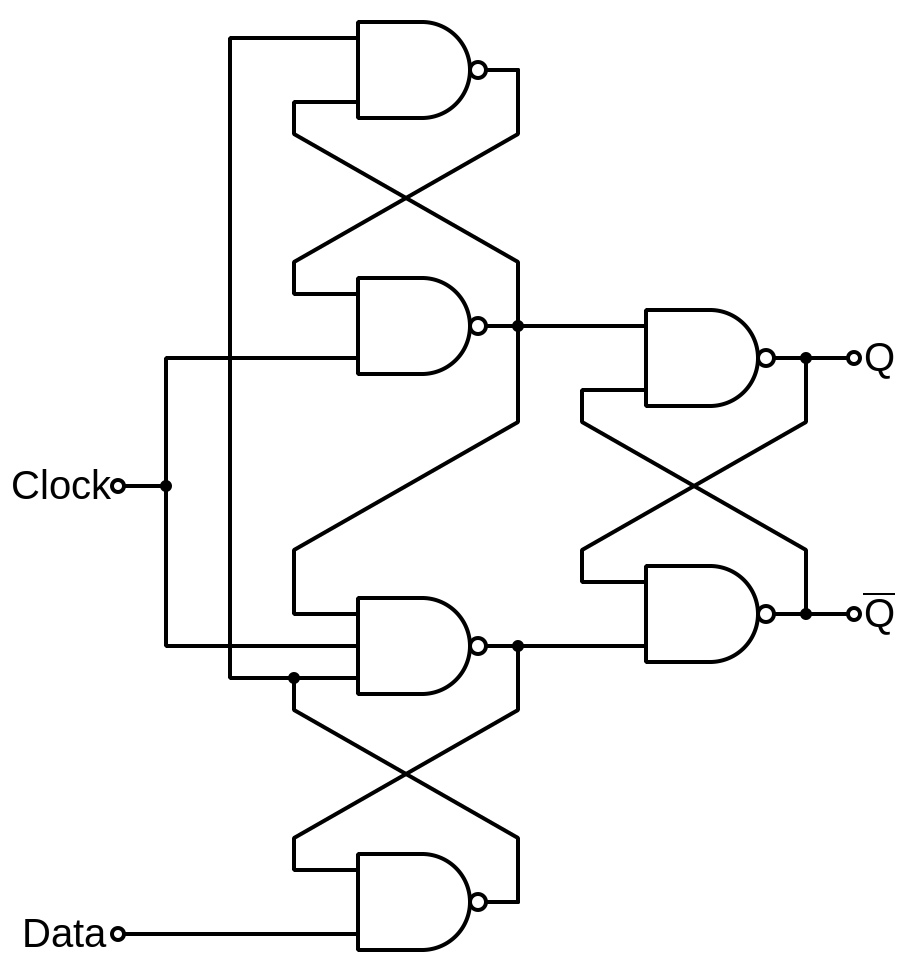
\includegraphics[height=7.5cm]{DFlipFlop.pdf}
    \subcaption{Classical D-type flip-flop built out of three $\overline{\text{SR}}$ NAND latches \cite{DFlipFlop}.}
  \end{subfigure}%
  \hspace{.05\textwidth}
  \begin{subfigure}[b]{.45\textwidth}
    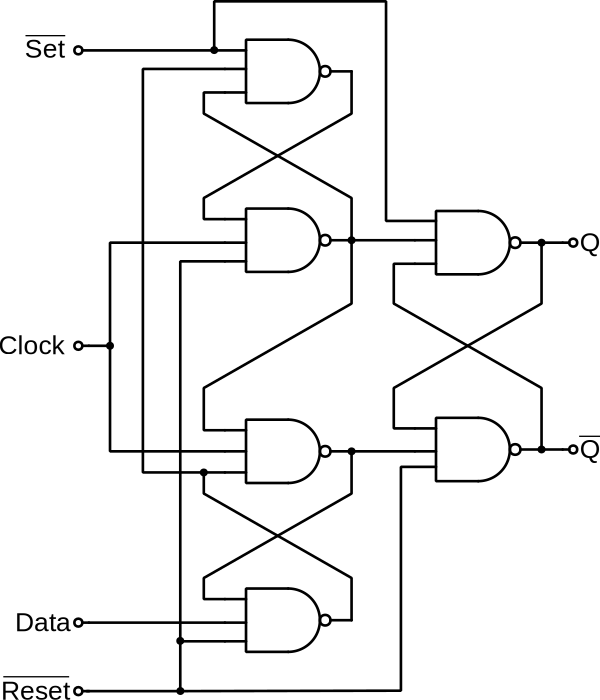
\includegraphics[height=7.5cm]{DFlipFlopClearSet.pdf}
    \subcaption{D-type flip-flop modified to support $\overline{\text{Clear}}$ and $\overline{\text{Set}}$ \cite{DFlipFlopClearSet}.}
  \end{subfigure}
  \caption{Comparison of D-type flip-flops with and without $\overline{\text{Clear}}$ and $\overline{\text{Set}}$.}
  \label{fig:clearSet}
\end{figure}
As the registers store the current state of execution, it is required that the registers start up to a known state.
Therefore, some registers feature a clear input (or set input) which forces all flip-flops to 0 (or 1).
This is usually accomplished by modifying the classical D-type flip-flop to allow for setting and resetting the internal $\overline{\text{SR}}$ NAND latches as shown in \cref{fig:clearSet}.

The third feature that may be important is a three-state output which allows the register to be directly connected to a bus.
It is accomplished by adding a tri-state output driver to the outputs of the flip-flops.

The logic \gls{IC} that was chosen for the \gls{EDiC} is the \emph{74F825} because it has all three features and is 8 bits wide.

\section{\gls{ALU} flags}\label{sec:aluFlags}
The original version had only two very basic flags: The zero flag and negative flag.
They are both very easy to derive and enable basic conditional execution.
However, when programming more complex applications it is desireable to be able to work with more advanced \gls{ALU} flags.
Having only Zero and Negative Flags, for example, does not allow unsigned operations which is especially important with only 8 data bits.
It limits unsigned operations to only 0-127 even though the \gls{ALU} would be capable of calculations with 0-256.

A lot of modern \glspl{CPU} feature many different flags with the Intel 64\textsuperscript{\textregistered} and IA-32 \gls{CPU} having about 20 different flags \cite[Section~3.4.3]{intelx86}.
However, the popular ARM Architecture has a rather unique but very capable system for conditional execution which relies on only the four most used \gls{ALU} flags.
The \gls{EDiC} uses the same flags and their functions are as follows:
\begin{itemize}
  \item \textbf{N} The \emph{Negative} flag indicates that the result is negative and is set if the 8th bit of the \gls{ALU} result is \texttt{'1'}.
  \item \textbf{Z} The \emph{Zero} flag indicates that the result is 0 and is set if all 8 result bits are 0.
  \item \textbf{V} The \emph{Overflow} flag indicates that an overflow occurred and is set if the carry in and carry out of the 8th full-adder are different.
  This detects arithmetic overflows for signed two's-complement calculations.
  \item \textbf{C} The \emph{Carry} flag is the carry out bit of the adder for adding and subtracting.
  For logical operations (\texttt{XOR} and \texttt{AND}) the carry flag has no meaning and for shifting operations it equals the last bit that was ``carried out'' (or is unchanged if shifting by 0 bits).
\end{itemize}

\section{16bit Addresses}
One of the major limitation of the 8 bit \gls{CPU} is the addressable memory space.
With only 8 bit for the memory address, the maximum amount of memory addressable is 256 bytes.
In the first version of the \gls{CPU} this limitation was extended a bit by providing 256 bytes of instruction memory besides 256 bytes of read only memory for instruction immediate values and 256 bytes of addressable \gls{SRAM}.
However, especially with a \gls{CISC} architecture, the limited \gls{SRAM} memory space limits the overall complexity of programs that can be done.
Additionally, more complex programs or even small operating systems are impossible to fit into 256 instructions.

Therefore, it was decided to extend the \gls{PC} and the memory addresses to 16 bit, which yields 65536 bytes of addressable \gls{SRAM} and theoretically 65536 instructions\footnote{The largest feasible \gls{EEPROM} available has only 15 address bits and with that only 32768 words of data.}.
It was decided to not extend the overall bus width to 16 bit because the architectural complexity of the design can increase exponentially with bus width.
However, this raises problems of where the 16 bit addresses come from.
This is addressed after explaining the other changes made to the memory module in \cref{sec:addrLogic}.

\section{Memory Mapped I/O}
Input and Output is one of the most important factors of any \gls{CPU} besides the computing capabilities which are mostly defined by the \gls{ALU}.
Using individual instructions for I/O which directly read from and write to the bus are limiting the usability quite a lot.
A common way to extend the I/O capabilities is to use so called Memory Mapped I/O.
This works by splitting the address space between actual memory and I/O devices.
Then every I/O operation is performed as a usual memory access but the memory chip does not receive the access and the I/O device addressed performs the operation.
In the \gls{EDiC} the memory address is decoded in such a way, that accesses to addresses \texttt{0xfe00} to \texttt{0xfeff} are performed by any connected I/O devices.
For this to work, the lower 8 address bits, the bus and memory control signals - i.e. write enable, read enable and I/O chip enable (active when the upper 8 address bits are \texttt{0xff}) - are exposed for I/O devices to connect to.
\section{Stack Implementation}
A feature that has been thoroughly missing from the first \gls{CPU} version is a kind of stack Implementation.
The stack is essential to the workings of the programming paradigm \emph{functions}.
When calling functions, the return address is usually (automatically) stored on the stack where also local variables can be stored.
This allows functions to be called recursively and also simplifies the written assembler compared to simple branching.

However, a typical stack implementation as in modern \glspl{CPU} architectures like ARM is rather complex.
It requires a \gls{SP} register which needs to be accessible like another general purpose register, including arithmetic operations which is not possible when the bus width is only 8 bits but the \gls{SP} is 16 bits wide.
Therefore, the \gls{EDiC} uses an unique approach to the stack:

Similarly to the memory mapped I/O it was decided to implement the stack as an 8 bit register which can be incremented and decremented.
Every time a memory access is performed where the upper 8 bits of the address equal \texttt{0xff}, a 17th address bit is set and the upper 8 address bits are replaced by the current value of the \gls{SP}.
For example: The \gls{SP}  is currently \texttt{0x21} and a memory access to the address \texttt{0xff42} is performed.
Then the actual address at the memory \gls{IC} is \texttt{0x1\_2142}.

This allows each function (which has a unique \gls{SP} value on the current call stack) to have 256 bytes of function local memory.
In the call instruction, the \gls{EDiC} automatically stores the return address at address \texttt{0xffff}, which is \texttt{0x1\_spff} after translation.
To store the whole 16 bit return address, a second memory \gls{IC} is used in parallel which only needs 256 bytes of storage.
In the hardware build of the \gls{EDiC} the same \gls{SRAM} \gls{IC} as for the main memory is used because it is cheaply available.
The call and return instructions are further described in \cref{sec:instructionSet}.
\TODO{explain function parameters}
\section{Addressing Logic}\label{sec:addrLogic}
With increasing the address width to 16 bit and also adding more functionality to the memory access, the addressing logic has become more complex.
There are two main sources for memory addresses: The new 16 bit \gls{MAR} which can be written to from the bus and the 16 bit instruction immediate.
As the bus is only 8 bits wide, there is a special instruction to write to the upper 8 bits of the \gls{MAR} and the lower bits are written in the memory access instruction.
This can be used when a memory address is stored in registers and is needed when looping through values in the memory like arrays.
When accessing addresses known at compile time, the instruction immediate can be used as an address which has been extended to support 16 bit.
These two sources of addresses are then decoded to either select the stack (upper 8 bits equal \texttt{0xff}), memory mapped I/O (\texttt{0xfe}) or regular memory access.
The chip enable of the main memory is only asserted when performing stack and regular memory accesses while the I/O chip enable is only asserted when the upper 8 bits are \texttt{0xfe}.
Additionally, the 17th address bit is asserted when stack access is performed and the upper 8 bits of the address are replaced with the \gls{SP} in this case.

\section{Debugging and Breakpoint}
An important feature when developing a \gls{CPU} is debugging capabilities.
The initial version could at least step the clock cycle by cycle.
As programs get complexer this feature quickly becomes less useful as each instruction is made of several cycles and when a problem occurs after several hundred instructions it is infeasible to step through all cycles.
Additionally, the usual application developer does not want to step through each cycle but rather step through each instruction, assuming that the instruction set works as intended.
Another important debugging feature is the use of breakpoints where the \gls{CPU} halts execution when the \gls{PC} reaches a specific address.

In the \gls{EDiC} halting was not realized by stopping the clock completely but rather by inhibiting the instruction step counter increment.
This has the advantage that the clock is not abruptly pulled to 0 or 1 and, therefore, no spikes on the clock line can occur.
To implement a cycle by cycle stepping mode, the halt signal is de-asserted for only one clock cycle.
To step whole instructions, the halt signal is de-asserted until the instruction is finished (marked by a control signal that is inserted at the end of each instruction from the control logic).
In breakpoint mode, the halt signal is controlled from a comparator that compares the \gls{PC} and a 16 bit user input, asserting the halt signal when those two equal.
As soon as the \gls{CPU} halts, the user can then switch to stepping mode and debug the specific instruction of the program.

\section{Final Instruction Set}\label{sec:instructionSet}
This section describes all available instructions, what they do and which instruction cycle performs which steps of the instruction.
Each instruction starts with the same two cycles for instruction fetching.
The following instructions are supported by the hardware:
\paragraph{\gls{ALU} operations}
The \gls{EDiC} supports a wide variety of instructions that perform \gls{ALU} operations.
All these operations take two arguments which are used for one of the possible operations shown in \cref{tab:aluOp}.
Each \gls{ALU} operation modifies the status flags.
\begin{itemize}
  \item \emph{Register x Register:} Takes two registers as parameter and the result is stored in the first parameter.

  Cycles:
  \begin{enumerate}
    \item Both register to \gls{ALU} A and B input, write enable of \gls{ALU} result register.
    \item Write content of \gls{ALU} result register into first parameter register.
  \end{enumerate}

  \item \emph{Register x Register (no write back):} Takes two registers as parameter and the result is only calculated for the status flags.

  Cycles:
  \begin{enumerate}
    \item Both register to \gls{ALU} A and B input, write enable of \gls{ALU} result register.
  \end{enumerate}

  \item \emph{Register x Memory (from Register):} Takes one register as \gls{ALU} A input and a second register which is used as a memory address for the \gls{ALU} B input.
  The result is stored in the first register.

  Cycles:
  \begin{enumerate}
    \item Second register is stored in the lower 8 bits of the \gls{MAR}\footnote{The upper 8 bits of the \gls{MAR} should be set beforehand}.
    \item Address calculations.
    \item First register and memory content as A and B inputs, write enable of the result register.
    \item Write content of \gls{ALU} result register into first parameter register.
  \end{enumerate}

  \item \emph{Register x Memory (from immediate):} Takes one register as \gls{ALU} A input and a 16 bit value as immediate which is used as a memory address for the \gls{ALU} B input.
  The result is stored in the first register.

  Cycles:
  \begin{enumerate}
    \item Address calculations.
    \item First register and memory content as A and B inputs, write enable of the result register.
    \item Write content of \gls{ALU} result register into first parameter register.
  \end{enumerate}

  \item \emph{Register x Memory (from immediate, no write back):} Takes one register as \gls{ALU} A input and a 16 bit value as immediate which is used as a memory address for the \gls{ALU} B input.
  The result is only calculated for the status flags.

  Cycles:
  \begin{enumerate}
    \item Address calculations.
    \item First register and memory content as A and B inputs, write enable of the result register.
  \end{enumerate}

  \item \emph{Register x Immediate:} Takes one register as \gls{ALU} A input and an 8 bit value as immediate  for the \gls{ALU} B input.
  The result is stored in the first register.

  Cycles:
  \begin{enumerate}
    \item Register and immediate value as A and B inputs and write enable of the result register.
    \item Write content of \gls{ALU} result register into first parameter register.
  \end{enumerate}

  \item \emph{Register x Immediate (no write back):} Takes one register as \gls{ALU} A input and an 8 bit value as immediate  for the \gls{ALU} B input.
  The result is only calculated for the status flags.

  Cycles:
  \begin{enumerate}
    \item Register and immediate value as A and B inputs and write enable of the result register.
  \end{enumerate}
\end{itemize}

\paragraph{Memory operations} Some \gls{ALU} operations also include reading values from memory.
However, the \gls{EDiC} features a lot more memory operations which are detailed below.
As all memory operations may perform memory mapped I/O operations, special care must be taken to allow asynchronous I/O devices to function as well.
This means that for each memory access, the address setup and hold must be an individual cycle, resulting in a 3 cycle memory access.
\begin{itemize}
  \item \emph{Load from register address:} Takes the second register parameter as the lower 8 bits of the memory address and writes the memory content to the first register.

  Cycles:
  \begin{enumerate}
    \item Second register to lower \gls{MAR}.
    \item Memory address setup.
    \item Memory read access and write back to first register.
    \item Memory address hold.
  \end{enumerate}

  \item \emph{Load from immediate address:} Takes a 16 bit immediate as the memory address and writes the memory content to the register.

  Cycles:
  \begin{enumerate}
    \item Memory address setup.
    \item Memory read access and write back to first register.
    \item Memory address hold.
  \end{enumerate}

  \item \emph{Load from immediate address with incremented \gls{SP}:} Takes a 16 bit immediate as the memory address and writes the memory content to the register.
  However, before the memory access, the \gls{SP} is incremented and after the access, the \gls{SP} is decremented again.
  This is used to access parameters for subfunctions.

  Cycles:
  \begin{enumerate}
    \item Increment Stack Pointer.
    \item Memory address setup.
    \item Memory read access and write back to first register.
    \item Memory address hold.
    \item Decrement Stack Pointer.
  \end{enumerate}

  \item \emph{Store to register address:} Takes the second register parameter as the lower 8 bits of the memory address and writes the content of the first register to the memory.

  Cycles:
  \begin{enumerate}
    \item Second register to lower \gls{MAR}.
    \item Memory address and data setup.
    \item Memory write access.
    \item Memory address and data hold.
  \end{enumerate}

  \item \emph{Store to immediate address:} Takes a 16 bit immediate as the memory address and writes the register content to memory.

  Cycles:
  \begin{enumerate}
    \item Memory address and data setup.
    \item Memory write access.
    \item Memory address and data hold.
  \end{enumerate}

  \item \emph{Store to immediate address with incremented \gls{SP}:} Takes a 16 bit immediate as the memory address and writes the register content to memory.
  However, before the memory access, the \gls{SP} is incremented and after the access, the \gls{SP} is decremented again.
  This is used to access parameters for subfunctions.

  Cycles:
  \begin{enumerate}
    \item Increment Stack Pointer.
    \item Memory address and data setup.
    \item Memory write access.
    \item Memory address and data hold.
    \item Decrement Stack Pointer.
  \end{enumerate}

  \item \emph{Set upper 8 bits of \gls{MAR} from register:} Sets the upper \gls{MAR} register to the content of the register.

  Cycles:
  \begin{enumerate}
    \item Register output enable and upper \gls{MAR} write enable.
  \end{enumerate}

  \item \emph{Set upper 8 bits of \gls{MAR} from immediate:} Sets the upper \gls{MAR} register to the 8 bit immediate value.

  Cycles:
  \begin{enumerate}
    \item Immediate output enable and upper \gls{MAR} write enable.
  \end{enumerate}
\end{itemize}

\paragraph*{Miscellaneous operations}
There are some more operations that are strictly speaking neither \gls{ALU} nor memory operations like moves and branches.
\begin{itemize}
  \item \emph{Move between register:} Set the first register to the value of the second.

  Cycles:
  \begin{enumerate}
    \item Second register output enable and first register write enable.
  \end{enumerate}

  \item \emph{Move immediate to register:} Set the register to the value of the immediate.

  Cycles:
  \begin{enumerate}
    \item Immediate output enable and first register write enable.
  \end{enumerate}

  \item \emph{Conditionally set \gls{PC} from immediate:} This is the only conditional operation available.
  Depending on the current status register the following cycles are either executed or \glspl{NOP} are executed.

  Cycles:
  \begin{enumerate}
    \item \gls{PC} write enable from immediate.
  \end{enumerate}

  \item \emph{Function Call:} Takes a 16 bit address which the \gls{PC} is set to.
  The \gls{SP} is incremented and the return address is stored on the stack.

  Cycles:
  \begin{enumerate}
    \item Increment \gls{SP} and write \texttt{0xffff} into the \gls{MAR}.
    \item Memory address and data (\gls{PC}) setup.
    \item Memory write access.
    \item Memory address and data hold.
    \item Load \gls{PC} from instruction immediate.
  \end{enumerate}

  \item \emph{Function Return:} Decrements the \gls{SP} and the \gls{PC} is loaded from the return address which is read from the memory.

  Cycles:
  \begin{enumerate}
    \item Write \texttt{0xffff} into the \gls{MAR}.
    \item Memory address setup.
    \item Memory read access and \gls{PC} write enable.
    \item Memory address hold.
    \item Decrement \gls{SP}.
  \end{enumerate}
\end{itemize}